\documentclass{article}

\usepackage[letterpaper, portrait, margin=1in]{geometry}
\usepackage{siunitx}
\usepackage{tikz}
\usepackage{mathtools}
\usetikzlibrary{shapes,backgrounds}
\usepackage{graphicx}
\usepackage{amsmath}

\setlength{\parindent}{0pt}

\begin{document}

\title{Dyanmics Equations for Smartmouse 2018}
\author{Peter Mitrano}

\maketitle

\section{Forward Kinematics}
Deriving the kinematic equations of a differential drive robot.

\hfill

\begin{figure}[h]
  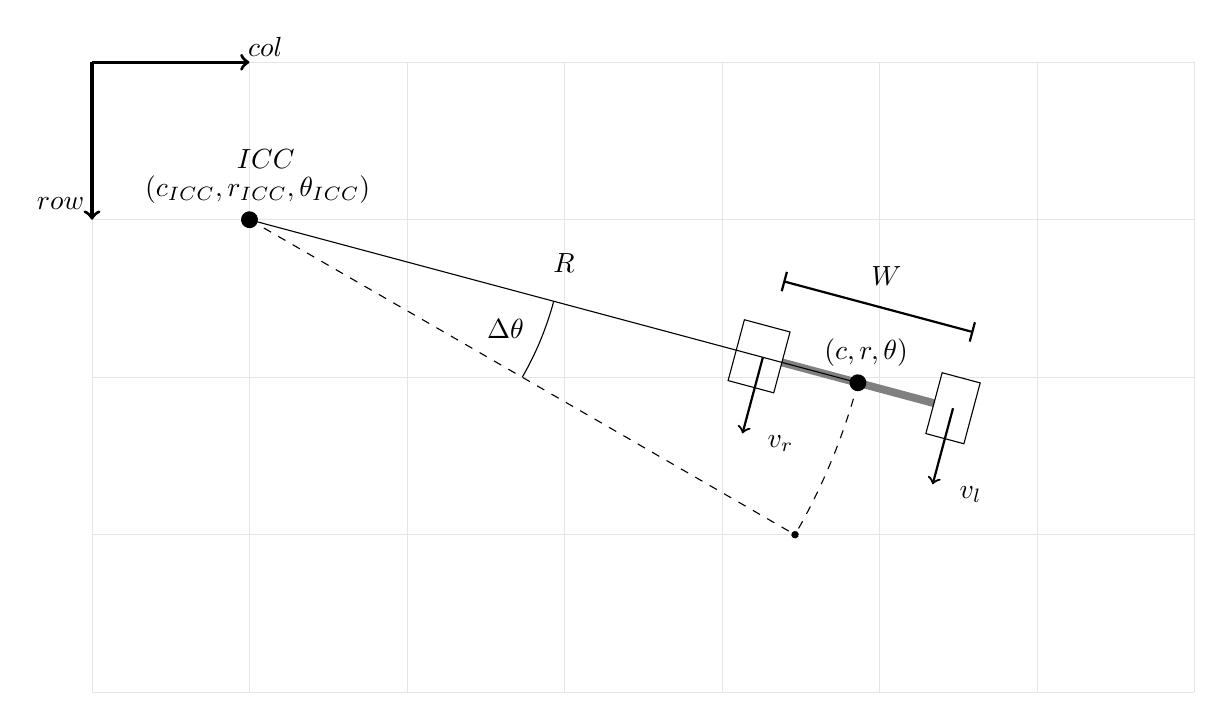
\begin{tikzpicture} [scale=2]
    % coordinate frame and grid%
    \definecolor{lg}{rgb}{0.9,0.9,0.9}
    \draw[step=1,lg,very thin] (-1,-3) grid (6,1);
    \draw [very thick,->] (-1,1) -- (-1,0);
    \draw [very thick,->] (-1,1) -- (0,1);
    \draw (-1.2, 0.1) node {$row$};
    \draw (0.1, 1.1) node {$col$};

    % robot and stuff %
    \draw [line width=1mm, draw=gray,rotate around={-15:(0,0)}]{(3.5,0)--(4.5, 0)};
    \draw [rotate around={-15:(0,0)}] {(3.2,-0.2) rectangle (3.5, 0.2)};
    \draw [rotate around={-15:(0,0)}] {(4.5,-0.2) rectangle (4.75, 0.2)};
    \draw [rotate around={-15:(0,0)}] {(0,0) -- (4, 0)};
    \draw [dashed,rotate around={-30:(0,0)}] {(0,0) -- (4, 0)};
    \draw [dashed,rotate around={-15:(0,0)}] (4,0) arc (0:-15:4);
    \draw [rotate around={-15:(0,0)}] (2,0) arc (0:-15:2);
    \draw [thick,->,rotate around={-15:(0,0)}] (3.375,0) -- (3.375,-0.5);
    \draw [thick,->,rotate around={-15:(0,0)}] (4.625,0) -- (4.625,-0.5);
    \draw [thick,|-|,rotate around={-15:(0,0)}] (3.375,0.5) -- (4.625,0.5);
    \filldraw [rotate around={-15:(0,0)}] {(0,0) circle (.05)};
    \filldraw [rotate around={-15:(0,0)}] {(4,0) circle (.05)};
    \filldraw [rotate around={-30:(0,0)}]{(4,0) circle (.02)};
    \draw [rotate around={-15:(0,0)}] (1.75, -0.25) node {$\Delta\theta$};
    \draw [rotate around={-15:(0,0)}] (3.625, -0.5) node {$v_r$};
    \draw [rotate around={-15:(0,0)}] (4.875, -0.5) node {$v_l$};
    \draw [rotate around={-15:(0,0)}] (2, 0.25) node {$R$};
    \draw [rotate around={-15:(0,0)}] (4, 0.7) node {$W$};
    \draw [rotate around={-15:(0,0)}] (4, .2) node {$(c,r,\theta)$};
    \draw [rotate around={-15:(0,0)}] (0, 0.4) node {$ICC$};
    \draw [rotate around={-15:(0,0)}] (0, .2) node {$(c_{ICC},r_{ICC},\theta_{ICC})$};
  \end{tikzpicture}
  \centering
\end{figure}

It's worth noting up front that we do not consider an X/Y plane. It is not a useful coordinate system for smartmouse. We think instead of row/column, where rows increase going down and columns increase going left to right. The top left cell is 0,0. Normally, we think of these as integer values, but we can also think of them as floating point values if we want to talk about the exact position in a cell. If you really want to, you can think of column as $x$ and row as $y$, with $z$ pointing down into the maze and positive angles going clockwise. With that out of the way, let's do the derivation.

At an instant in time we say that the robot is turning around some point $ICC$, the instanteous center of curvature. The radius $R$ about that point is what we want to solve for. We start with the knowedge that since the robot doesn't tear itself apart while driving, the rate $\omega$ at which both wheels (and the robot) move around $ICC$ is the same.
\begin{equation} \label{eq:1}
  \omega_l = \omega_r = \omega
\end{equation}
Let $R_l$ and $R_l$ be the radius to the right and left wheels.
\begin{equation} \label{eq:2}
  \omega = \frac{v_l}{R_l} = \frac{v_r}{R_r}
\end{equation}
We can then combine \ref{eq:1} and \ref{eq:2}
\begin{equation}
  \frac{v_l}{R_l} = \frac{v_r}{R_r}
\end{equation}
We can then substitute $R_l = R + \frac{W}{2}$ and $R_r = R - \frac{W}{2}$
\begin{equation}
  \frac{v_l}{R+\frac{W}{2}} = \frac{v_r}{R-\frac{W}{2}}
\end{equation}

Now do some algebra...
\begin{align*}
  \frac{v_l}{R+\frac{W}{2}} &= \frac{v_r}{R-\frac{W}{2}} \\[1em]
  \frac{R+\frac{W}{2}}{v_l} &= \frac{R-\frac{W}{2}}{v_r} \\[1em]
  \frac{R}{v_l}+\frac{W}{2v_l} &= \frac{R}{v_r}-\frac{W}{2v_r} \\[1em]
  \frac{W}{2v_l} + \frac{W}{2v_r} &= \frac{R}{v_r} - \frac{R}{v_l} \\[1em]
  \frac{W(v_r + v_l)}{2v_rv_l} &= \frac{R(v_l - v_r)}{v_rv_l} \\[1em]
  \frac{W(v_r + v_l)}{2(v_l - v_r)} &= R
\end{align*}

We can use this result to get a cleaner equation for $\omega$, which right now requires diving by $R$. This is problematic because $R$ can be $0$.

\begin{align*}
  \omega &= \frac{v_l}{R+\frac{W}{2}}\\[1em]
         &= \frac{v_l}{\frac{W(v_r+v_l)}{2(v_l - v_r)}+\frac{W}{2}}\\[1em]
         &= \frac{v_l}{\frac{W(v_r+v_l)}{2(v_l - v_r)}+\frac{W(v_l - v_r)}{2(v_l - v_r)}}\\[1em]
         &= \frac{v_l}{\frac{W(v_r+v_l)+W(v_l - v_r)}{2(v_l - v_r)}}\\[1em]
         &= \frac{2v_l(v_l - v_r)}{W(v_r+v_l)+W(v_l - v_r)}\\[1em]
         &= \frac{2v_l(v_l - v_r)}{Wv_r+Wv_l+Wv_l-Wv_r}\\[1em]
         &= \frac{2v_l(v_l - v_r)}{2Wv_l}\\[1em]
         &= \frac{v_l - v_r}{W} [1em]
\end{align*}


\textbf{Next we need to figure out how to update our $c$, $r$, and $\theta$ given $R$.} \\

Before we can solve any of these, we need to figure out what $\Delta\theta$ is equal to. We will assume we are following this arc of constant radius for a given time step $\Delta t$. This is a good assumption if our time step is equal to our controller time step, during which presumably the speeds of the motors aren't changing, and so neither will our turning radius. If so, then $\Delta\theta = \omega\Delta t$, and we know

$$\omega=\frac{v_l - v_r}{W}$$

Lets just pick $v_l$, and put them together to get $\Delta\theta$.

$$\Delta\theta = \frac{v_l - v_r}{W}\Delta t$$

So what are our update equations? \\

Theta is obvious: $\theta \leftarrow \theta+\Delta\theta$. \\

To discover the rest, we will consider how to c and r change when we rotate around the $ICC$. \\

The coordinates of the $ICC$ are:

$$(c_{ICC}, r_{ICC}) = (c-R\sin{\theta}, r+R\cos{\theta})$$

You can see this if you think that the vector to $ICC$ is 90 degrees offset from $\theta$ and do the trig. Let's assume in the situation diagramed above, $\theta=\ang{105}$, $R=4$, and $c=4.8, r=2$, so $ICC = (4.8-4\sin{(105)}, 2+4\cos{(105)}) \approx (1, 1)$. For another example, pretend the robot is right below the origin facing east at $(0,1,0)$ and $R=-1$. $ICC$ should be $(0,0)$ so let's check. $ICC = (0-{-1}\sin{(0)}, 1+{-1}\cos{(0)}) = (0, 0).$ Great, the math seems to check out. Now we just rotate the robot coordinates around the point $ICC$ by $\Delta\theta$, which we can do easily with a rotation matrix. Of course, we're not rotating around the origin, we're roating around $ICC$, so we first subtract out the coordinates of $ICC$ to get $(c_o, r_o) = (c-c_{ICC}, r-r_{ICC})$. Recall that to rotate around the origin by $\Delta\theta$, we multiply our point $(c_o, r_o)$ as follows.
\begin{equation}
  \begin{bmatrix}
    \cos{\Delta\theta} & -\sin{\Delta\theta} \\
    \sin{\Delta\theta} & \cos{\Delta\theta} \\
  \end{bmatrix}
  \begin{bmatrix}
    c_o \\
    r_o \\
  \end{bmatrix}
  =
  \begin{bmatrix}
    c_{new} \\
    r_{new} \\
  \end{bmatrix}
\end{equation}
We then just add back the coordinates of $ICC$. Great! Now we know how to update all our coordinates. Let's summarize:

\begin{align}
 \theta &\leftarrow \theta + \Delta\theta \\
  c &\leftarrow \cos{(\Delta\theta)}(c-c_{ICC})-\sin{(\Delta\theta)}(r-r_{ICC}) + c_{ICC} \\
  r &\leftarrow \sin{(\Delta\theta)}(c-c_{ICC})+\cos{(\Delta\theta)}(r-r_{ICC}) + r_{ICC} \\
\shortintertext{where}
  c_{ICC} &= c-R\sin{\theta} \\
  r_{ICC} &= r+R\cos{\theta} \\
  \Delta\theta &= \frac{v_l-v_r}{W}\Delta t \\
  R &= \frac{W(v_r+v_l)}{2(v_l-v_r)}
\end{align}

We can expand and simplify the update equations for $c$.

\begin{align}
  c &\leftarrow \cos{(\frac{v_l-v_r}{W}\Delta t)}(c-(c-R\sin{\theta}))-\sin{(\frac{v_l-v_r}{W}\Delta t)}(r-(r+R\cos{\theta})) + c-R\sin{\theta} \\
  c &\leftarrow \cos{(\frac{v_l-v_r}{W}\Delta t)}(c-c+R\sin{\theta})-\sin{(\frac{v_l-v_r}{W}\Delta t)}(r-r-R\cos{\theta}) + c-R\sin{\theta} \\
  c &\leftarrow \cos{(\frac{v_l-v_r}{W}\Delta t)}(R\sin{\theta})-\sin{(\frac{v_l-v_r}{W}\Delta t)}(-R\cos{\theta}) + c-R\sin{\theta} \\
  c &\leftarrow R\cos{(\frac{v_l-v_r}{W}\Delta t)}\sin{\theta}+R\sin{(\frac{v_l-v_r}{W}\Delta t)}\cos{\theta} + c-R\sin{\theta} \\
  c &\leftarrow c+R\cos{(\frac{v_l-v_r}{W}\Delta t)}\sin{\theta}+R\sin{(\frac{v_l-v_r}{W}\Delta t)}\cos{\theta}-R\sin{\theta} \\
  c &\leftarrow c+R\Big(\cos{(\frac{v_l-v_r}{W}\Delta t)}\sin{\theta}+\sin{(\frac{v_l-v_r}{W}\Delta t)}\cos{\theta}\Big)-R\sin{\theta} \\
  \shortintertext{let $\frac{v_l-v_r}{W}=a$, and $\theta=b$, we can use $\cos{a}\sin{b}+\sin{a}\cos{b}=\sin{(a+b)}$}
  c &\leftarrow c+R\Bigg(\sin{\Big(\frac{v_l-v_r}{W}\Delta t+\theta}\Big)\Bigg)-R\sin{\theta} \\
  c &\leftarrow c+R\Bigg(\sin{\Big(\frac{v_l-v_r}{W}\Delta t+\theta}\Big)-\sin{\theta}\Bigg)
\end{align}

We can apply the same process for $r$.

\begin{align}
  r &\leftarrow \sin{(\frac{v_l-v_r}{W}\Delta t)}(c-(c-R\sin{\theta}))+\cos{(\frac{v_l-v_r}{W}\Delta t)}(r-(r+R\cos{\theta})) + r+R\cos{\theta} \\
  r &\leftarrow \sin{(\frac{v_l-v_r}{W}\Delta t)}(c-c+R\sin{\theta})+\cos{(\frac{v_l-v_r}{W}\Delta t)}(r-r-R\cos{\theta}) + r+R\cos{\theta} \\
  r &\leftarrow \sin{(\frac{v_l-v_r}{W}\Delta t)}(R\sin{\theta})+\cos{(\frac{v_l-v_r}{W}\Delta t)}(-R\cos{\theta}) + r+R\cos{\theta} \\
  r &\leftarrow R\sin{(\frac{v_l-v_r}{W}\Delta t)}(\sin{\theta})-R\cos{(\frac{v_l-v_r}{W}\Delta t)}(\cos{\theta}) + r+R\cos{\theta} \\
  r &\leftarrow r + R\sin{(\frac{v_l-v_r}{W}\Delta t)}(\sin{\theta})-R\cos{(\frac{v_l-v_r}{W}\Delta t)}(\cos{\theta}) + R\cos{\theta} \\
  r &\leftarrow r + R\Big(\sin{(\frac{v_l-v_r}{W}\Delta t)}(\sin{\theta})-\cos{(\frac{v_l-v_r}{W}\Delta t)}(\cos{\theta}\Big) + R\cos{\theta} \\
  \shortintertext{let $\frac{v_l-v_r}{W}=a$, and $\theta=b$, we can use $\sin{a}\sin{b}-\cos{a}\cos{b}=-\cos{(a+b)}$}
  r &\leftarrow r - R\Bigg(\cos{\Big(\frac{v_l-v_r}{W}\Delta t + \theta\Big)}\Bigg) + R\cos{\theta} \\
  r &\leftarrow r - R\Bigg(\cos{\Big(\frac{v_l-v_r}{W}\Delta t + \theta\Big)} - \cos{\theta}\Bigg)
\end{align}

\textbf{Final Solution to the forward Kinematics:}
\begin{align}
 \theta &\leftarrow \theta + \frac{v_l-v_r}{W}\Delta t \\
  c &\leftarrow c + R\Bigg(\sin{\Big(\frac{v_l-v_r}{W}\Delta t+\theta\Big)}-\sin{\theta}\Bigg) \\
  r &\leftarrow r + -R\Bigg(\cos{\Big(\frac{v_l-v_r}{W}\Delta t+\theta\Big)}-\cos{\theta}\Bigg)
\end{align}

However, there is also the case where the robot is going perfectly straight. This has to be handled seperately, because otherwise the equations above involve $R$, but $R=\infty$ if we're going straight. Luckily, the equations for moving straight are trivial:
\begin{align}
 \theta &\leftarrow \theta \\
  c &\leftarrow c + v\Delta t\cos(theta) \\
  r &\leftarrow r - v\Delta t\sin(theta)
\end{align}

Here, $v$ can be $v_l$, or $v_r$ since they should be the same. In code, a simple average is used to correct for any slight numerical inconsistencies. \\

\section{DC Motor Modeling}
We must also consider how to model the DC Motors. \\

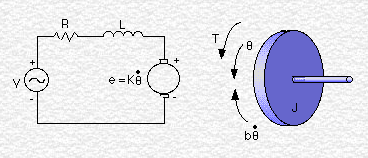
\includegraphics[scale=0.5]{./dc_motor_model.png}

The motor torque, $T$, is related to the armature current, $i$, by a constant factor $K$. The back emf, $e$, is related to the rotational velocity by the following equations:
$$T=Ki$$
$$e=K\dot{\theta}$$

From the figure above we can write the following equations based on Newton's law combined with Kirchhoff's law:
$$J\frac{d}{dt}\dot{\theta} + b\dot{\theta} = Ki$$
$$L\frac{d}{dt}i+Ri=V-K\dot{\theta}$$

In state-space form, the equations above can be expressed by choosing the rotating speed and electric current as the state variables and the voltage as an input. The output is chosen to be the rotating speed. The general linear state-space form is $\dot{X} = AX + BW$. We can get the two equations above in this form with some algebra.
\begin{align}
  J\frac{d}{dt}\dot{\theta} + b\dot{\theta} &= Ki \\
  \frac{d}{dt}\dot{\theta} + \frac{b\dot{\theta}}{J} &= \frac{Ki}{J} \\
  \frac{d}{dt}\dot{\theta} &= \frac{Ki}{J} - \frac{b\dot{\theta}}{J}
\end{align}

\begin{align}
  L\frac{d}{dt}i + Ri &= V - K\dot{\theta} \\
  \frac{d}{dt}i + \frac{Ri}{L} &= \frac{V}{L} - \frac{K\dot{\theta}}{L} \\
  \frac{d}{dt}i &= \frac{V}{L} - \frac{K\dot{\theta}}{L} - \frac{Ri}{L}
\end{align}

Next we combine these in a matrix.

\begin{align}
  \frac{d}{dt}\begin{bmatrix}\dot{\theta}\\i\\\end{bmatrix} &=
    \begin{bmatrix}
      \frac{-b}{J} & \frac{K}{J} \\
      \frac{-K}{L} & \frac{-R}{L} \\
    \end{bmatrix}
    \begin{bmatrix}
      \dot{\theta} \\
      i
    \end{bmatrix}
    +
    \begin{bmatrix}
      0 \\
      \frac{1}{L}
    \end{bmatrix}
    V
\end{align}

What this gives us is a nice matrix-y formula for the change in the current and angle of our motor over time. We can use this equation to simulate the behavior of the motor. If we assume the motor start at some initial $\dot{\theta}$, $i_0$ and $\dot{i}$, and we know all our motor constants ($K$, $R$, $L$, $b$, $J$) we can figure out the right hand side of the equation, and the result will be how much $i$ and $\dot{\theta}$ changes over some discrete time step. That is what we do in the smartmouse simulator server code.

\end{document}

